\documentclass[]{article}
\usepackage[T1]{fontenc}
\usepackage[polish]{babel}
\usepackage[utf8]{inputenc}
\usepackage{graphicx}
\graphicspath{ {images/} }

%opening
\title{Sortowanie klocków LEGO}
\author{}

\begin{document}
	
	\maketitle
	
	\begin{abstract}
		
	\end{abstract}
	
	\section{Założenia etapu}
	Celem etapu było zbudowanie aplikacji na Androida, której główną funkcją jest robienie zdjęć klocków Lego oraz przesyłanie ich na serwer, gdzie następnie klocki są wycinane oraz poddawane klasyfikacji. Podczas prac nad projektem, wstępne założenia zostały rozszerzone, by przyspieszyć prace nad generowaniem datasetu. 
	Niniejszy raport dzieli się na sekcje, które opisują aplikację, serwer, detekcję klocków Lego oraz ich klasyfikację.
	Do raportu dołączone są nagrania, pokazujące działanie wszystkich zaimplementowanych funkcji.  
	
	\section{Aplikacja mobilna}
	Aplikacja mobilna pełni rolę przechwytywania zdjęć klocków Lego oraz wysyłania ich na serwer. Połączenie między aplikacją i serwerem jest zrealizowane przy użyciu gRPC. 
	Możemy wyróżnić dwa tryby, w których działa aplikacja
	\begin{itemize}
		\item Analyze - tryb, w którym aplikacja wysyła na serwer zdjęcia w niskiej jakości, które następnie są przetwarzane przez serwer, a odpowiedź z serwera zawiera informacje o położeniu klocków oraz rozpoznanych klasach. \\
		Zapytania do serwera są blokujące, z tego powodu obraz nie jest płynny i dostrzegalne są małe opóźnienia w odpowiedziach. W celu zminimalizowania opóźnień, zdjęcia są w rozdzielczości niższej niż 1080 x 1080px.
		\item Capture - tryb, którego głównym celem w trakcie pisania tego raportu jest tworzenie datasetu z klockami Lego. Zdjęcia są w najwyższej możliwej jakości obsługiwanej przez telefon, a zapytania do serwera są nieblokujące. Tryb jest konfigurowalny, co pozwala na ustawienie interwału robienia zdjęć, przejście do trybu ręcznego a także określenie klasy klocków, jakie są aktualnie fotografowane.
	\end{itemize}
	
	
	\begin{figure}[h!]
		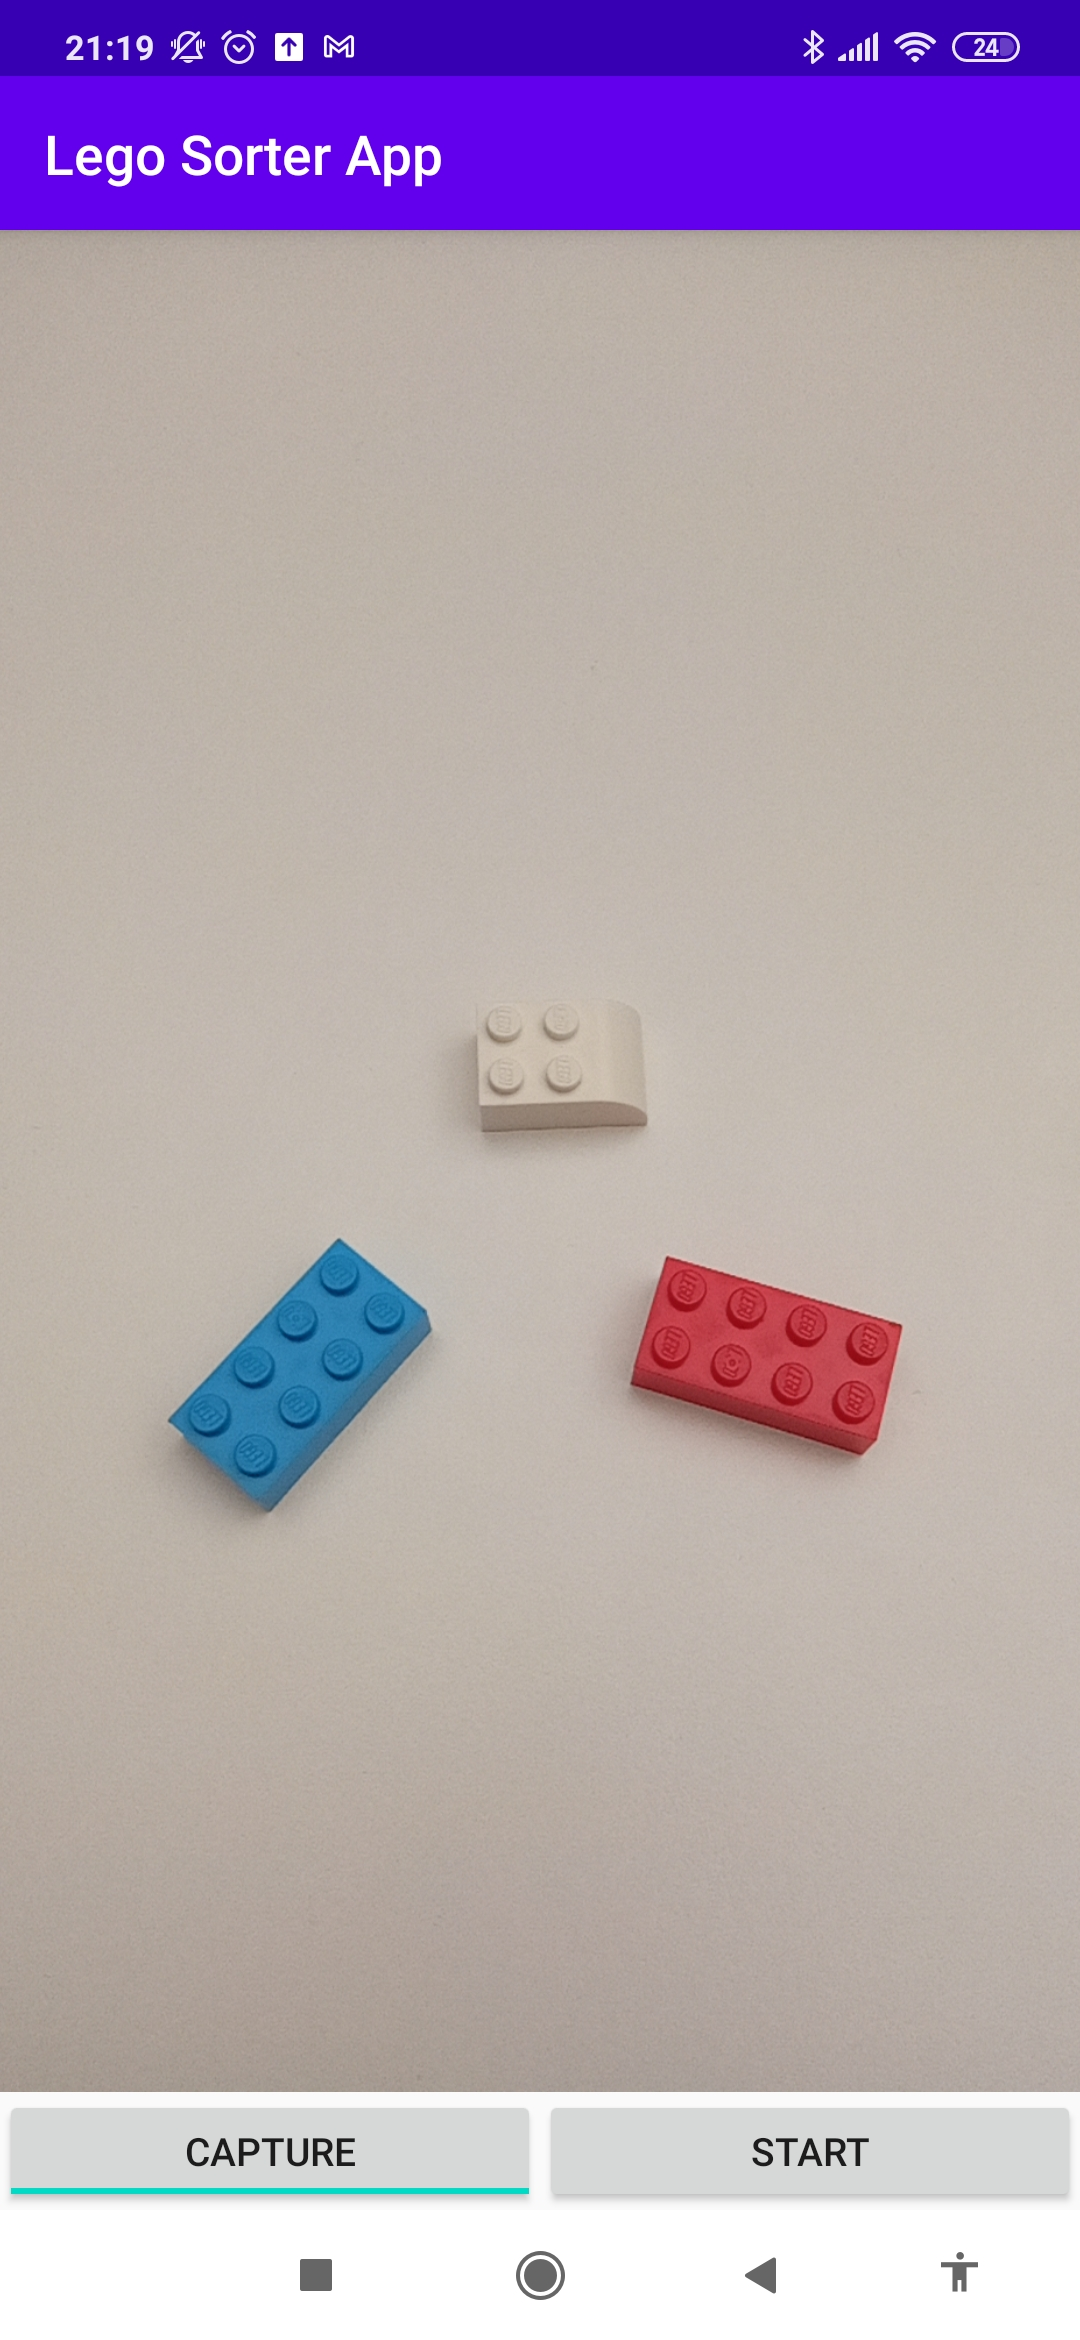
\includegraphics[width=0.3\linewidth]{main_view}
		\centering
		\caption{Główny ekran aplikacji pozwala na wybranie trybu robienia zdjęć.}
	\end{figure}
	
	\begin{figure}[h!]
		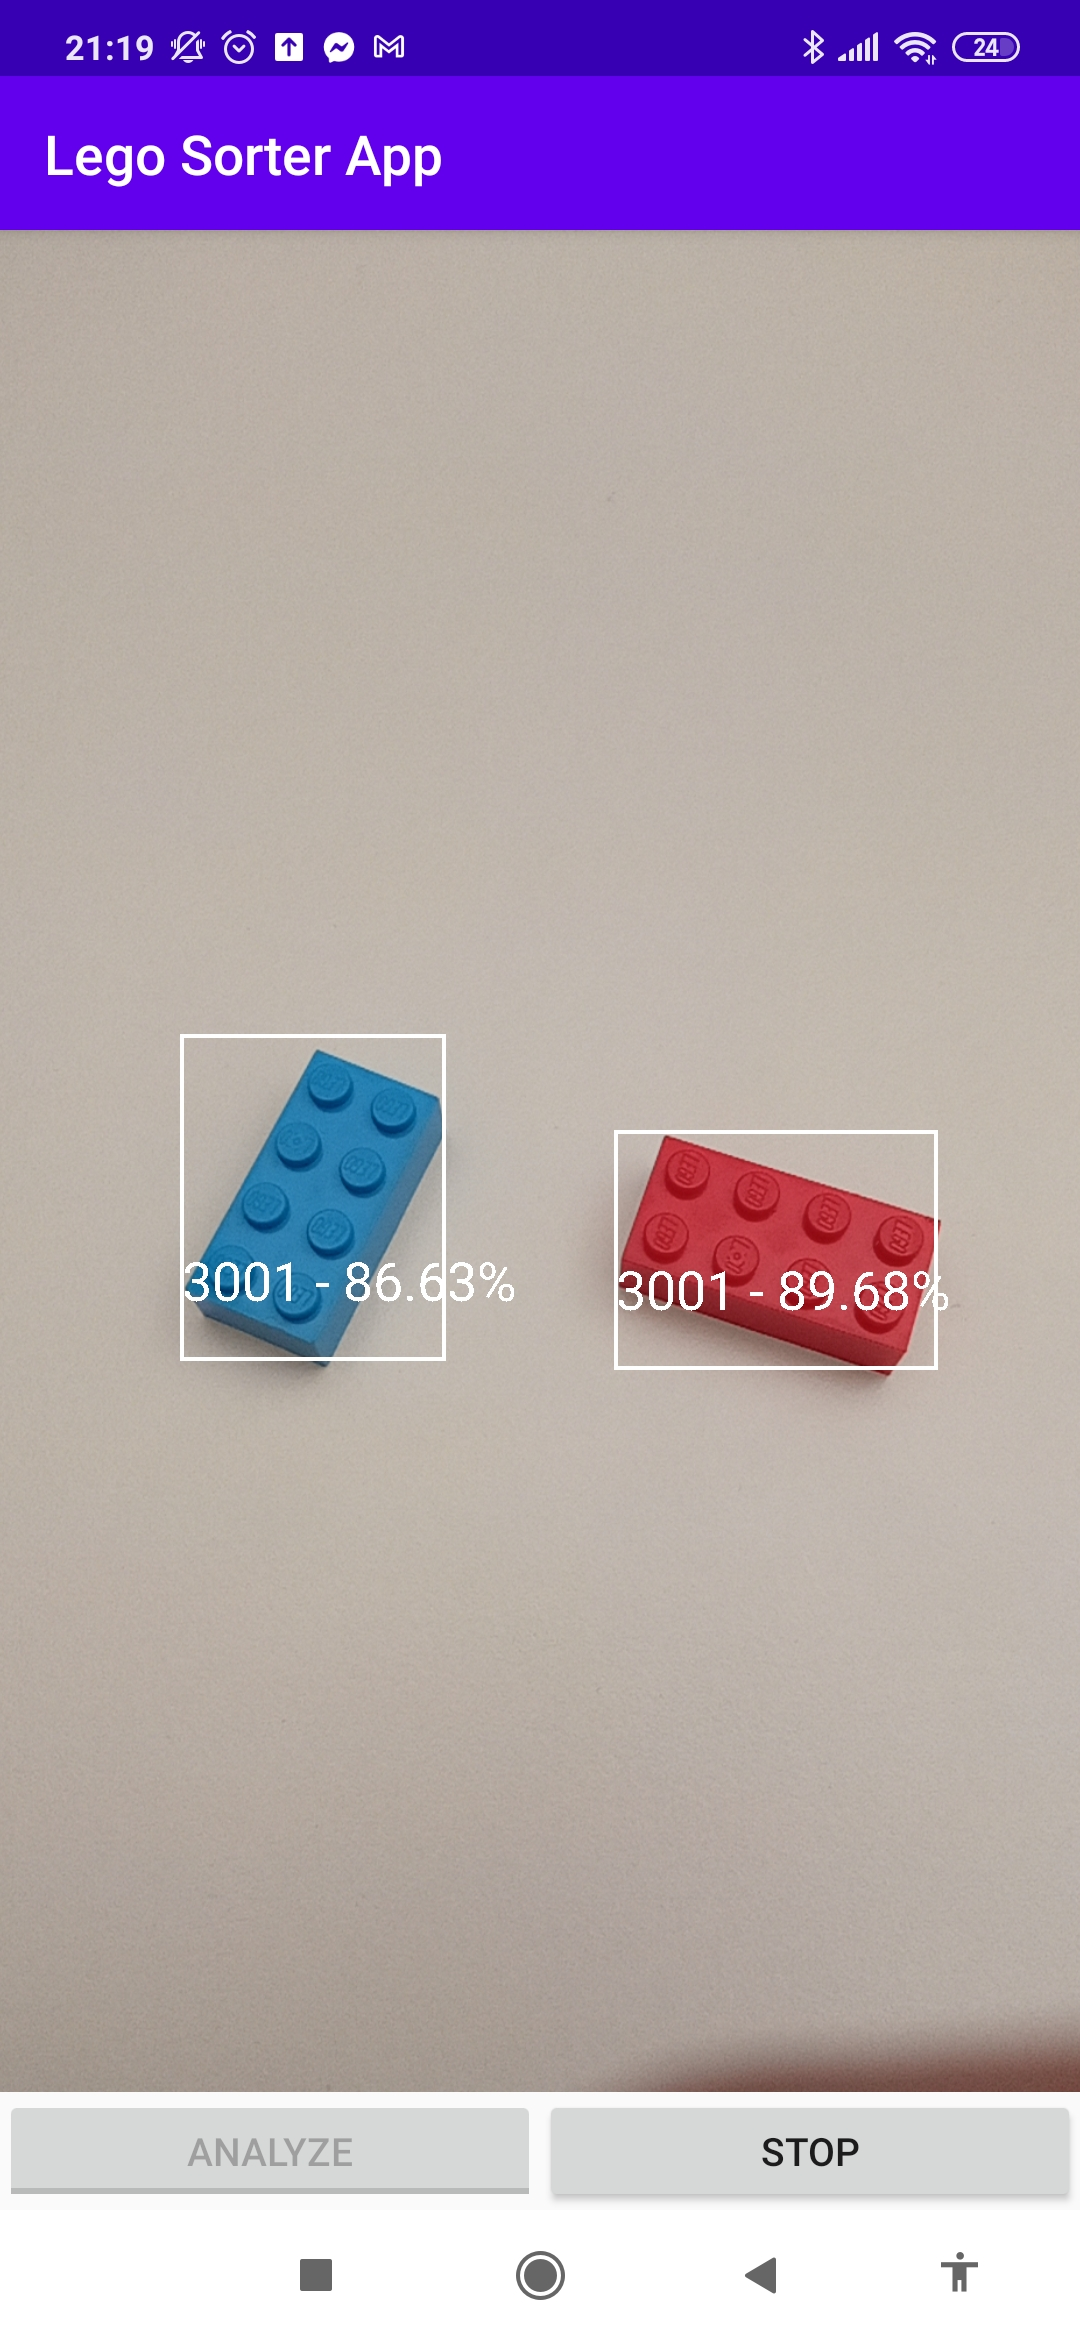
\includegraphics[width=0.3\linewidth]{analyze_view}
		\centering
		\caption{Widok analyze pokazuje wykryte klocki oraz przypisane do nich klasy}
	\end{figure}
	
	\begin{figure}[h!]
		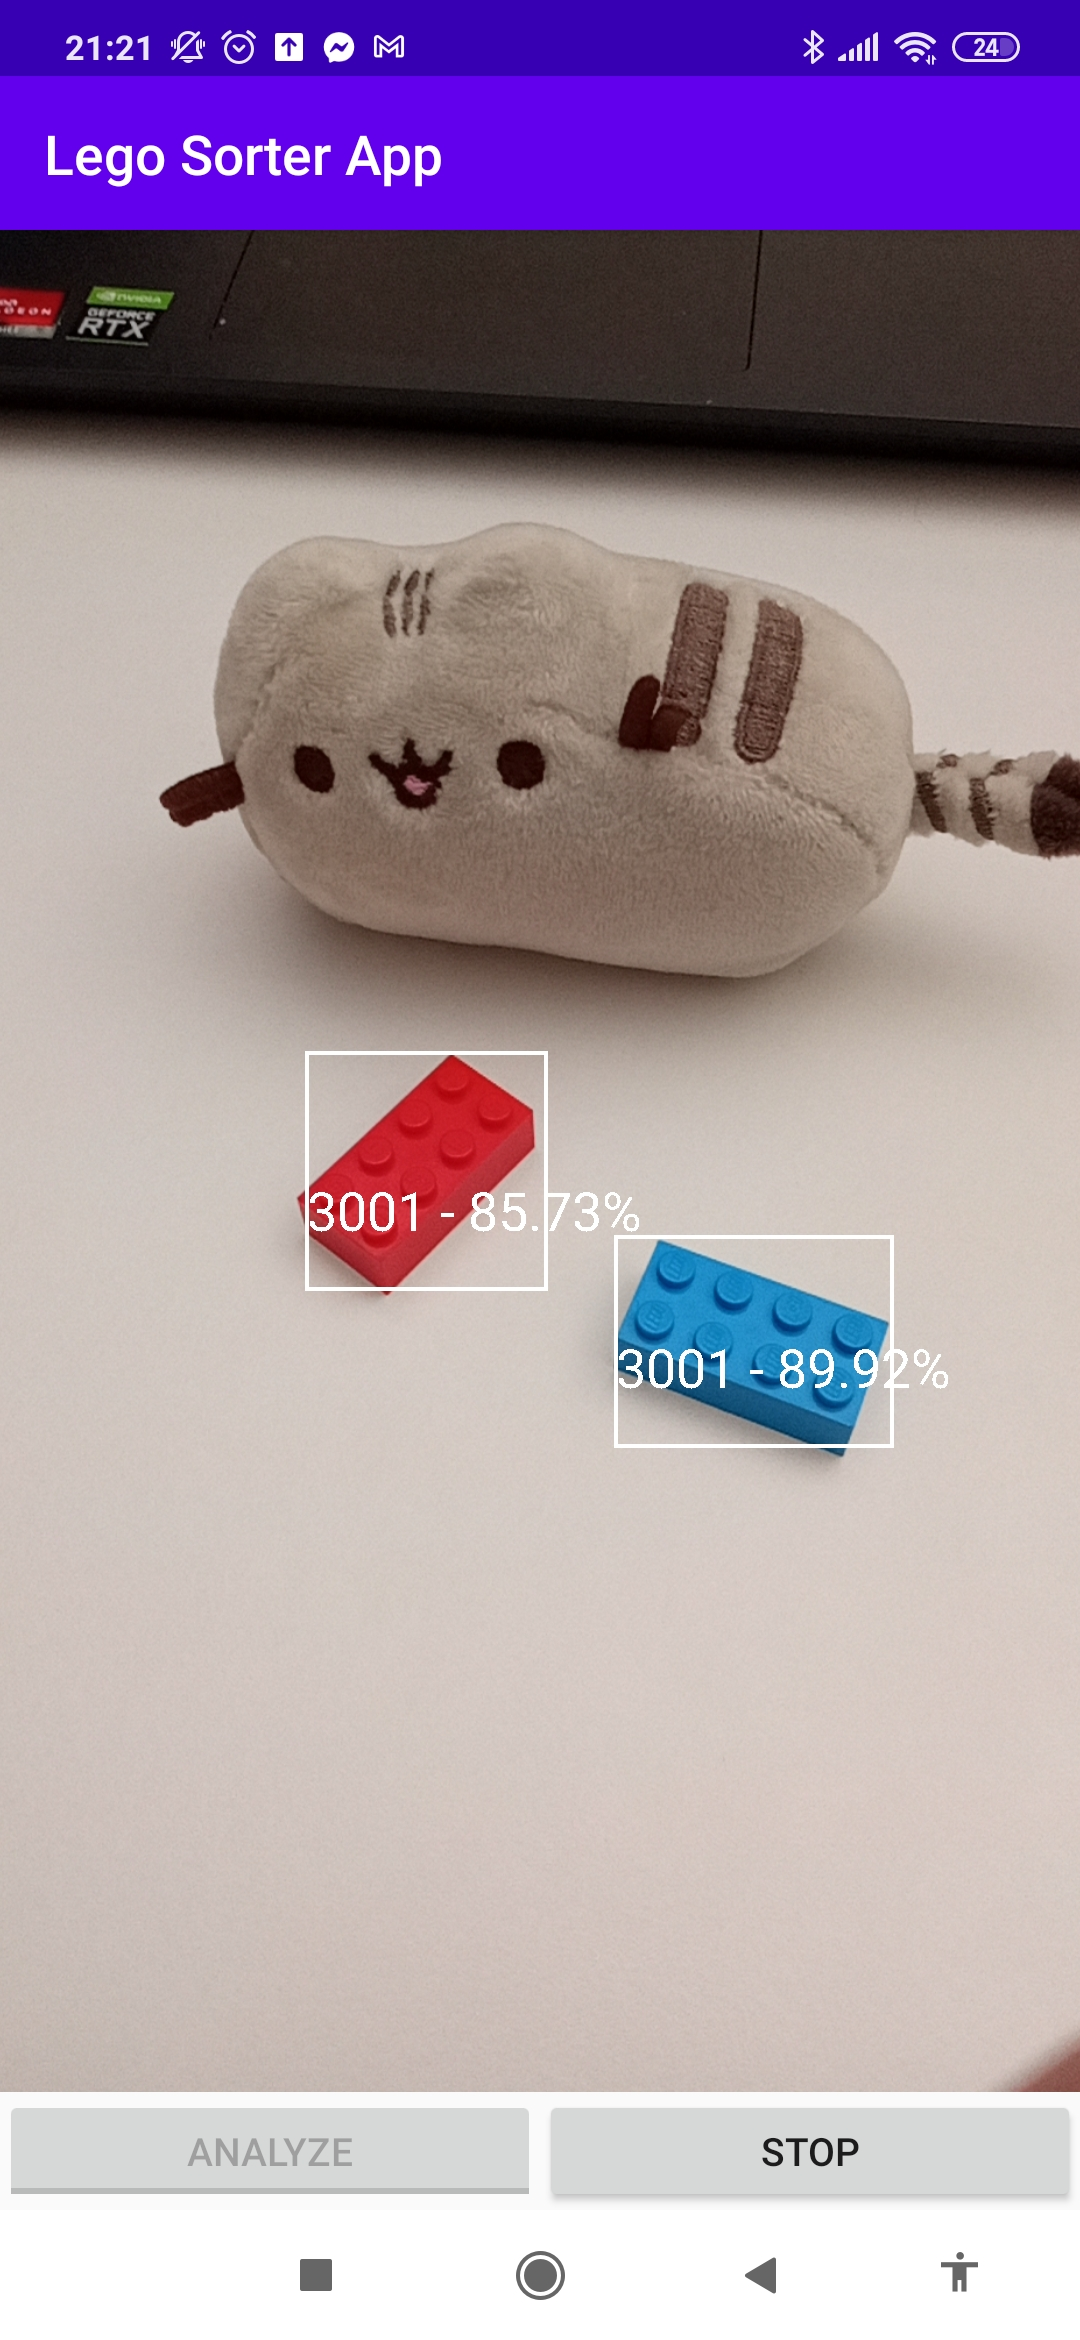
\includegraphics[width=0.3\linewidth]{analyze_view_2}
		\centering
		\caption{Obiekty, które nie zostały rozpoznane jako klocki lego, są pomijane}
	\end{figure}
	
	\begin{figure}[h!]
		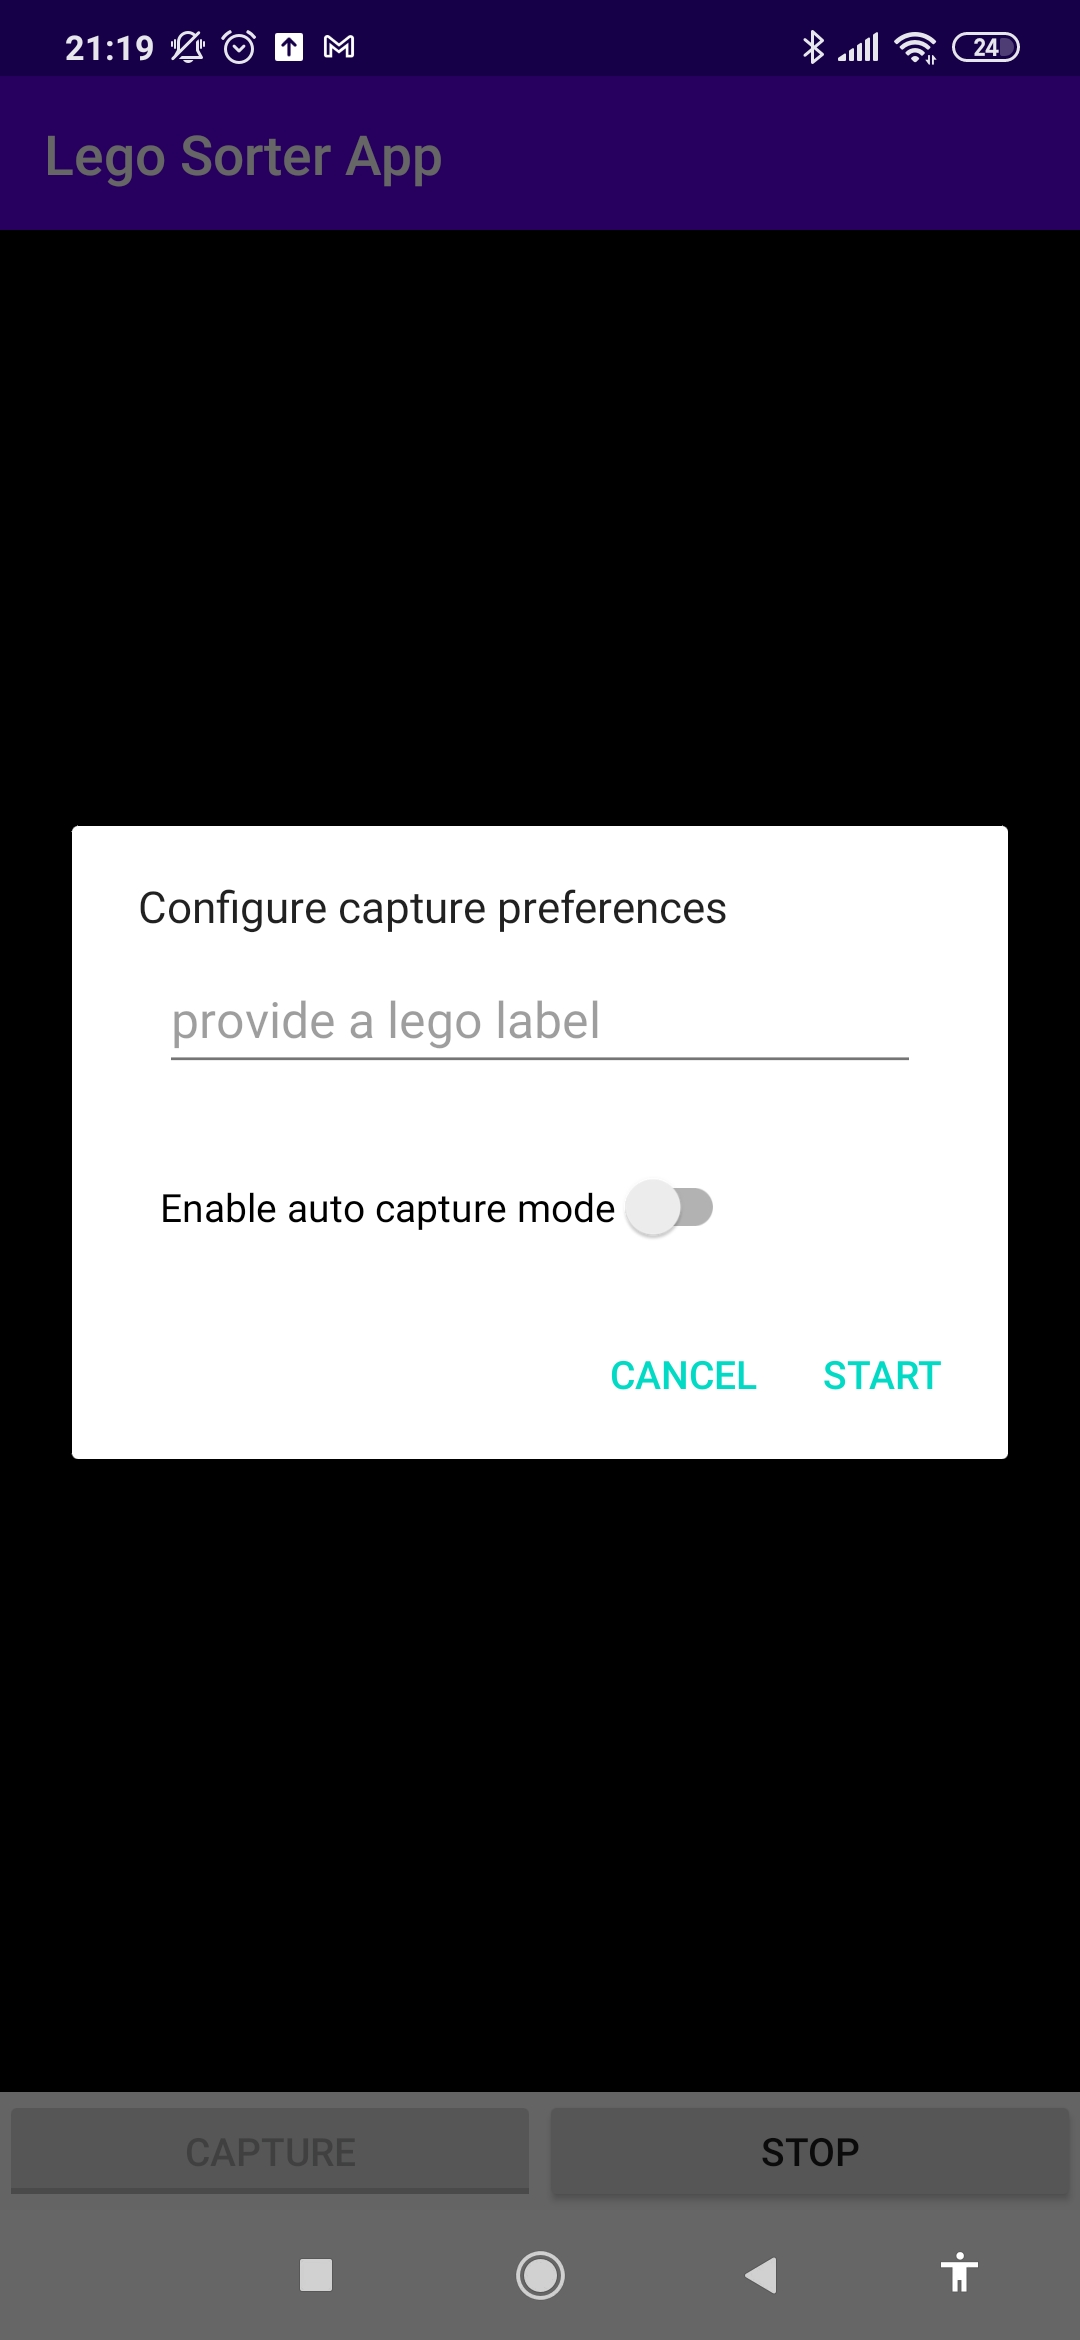
\includegraphics[width=0.3\linewidth]{capture_preferences}
		\centering
		\caption{Tryb capture udostępnia okno preferencji}
	\end{figure}
	
	\begin{figure}[h!]
		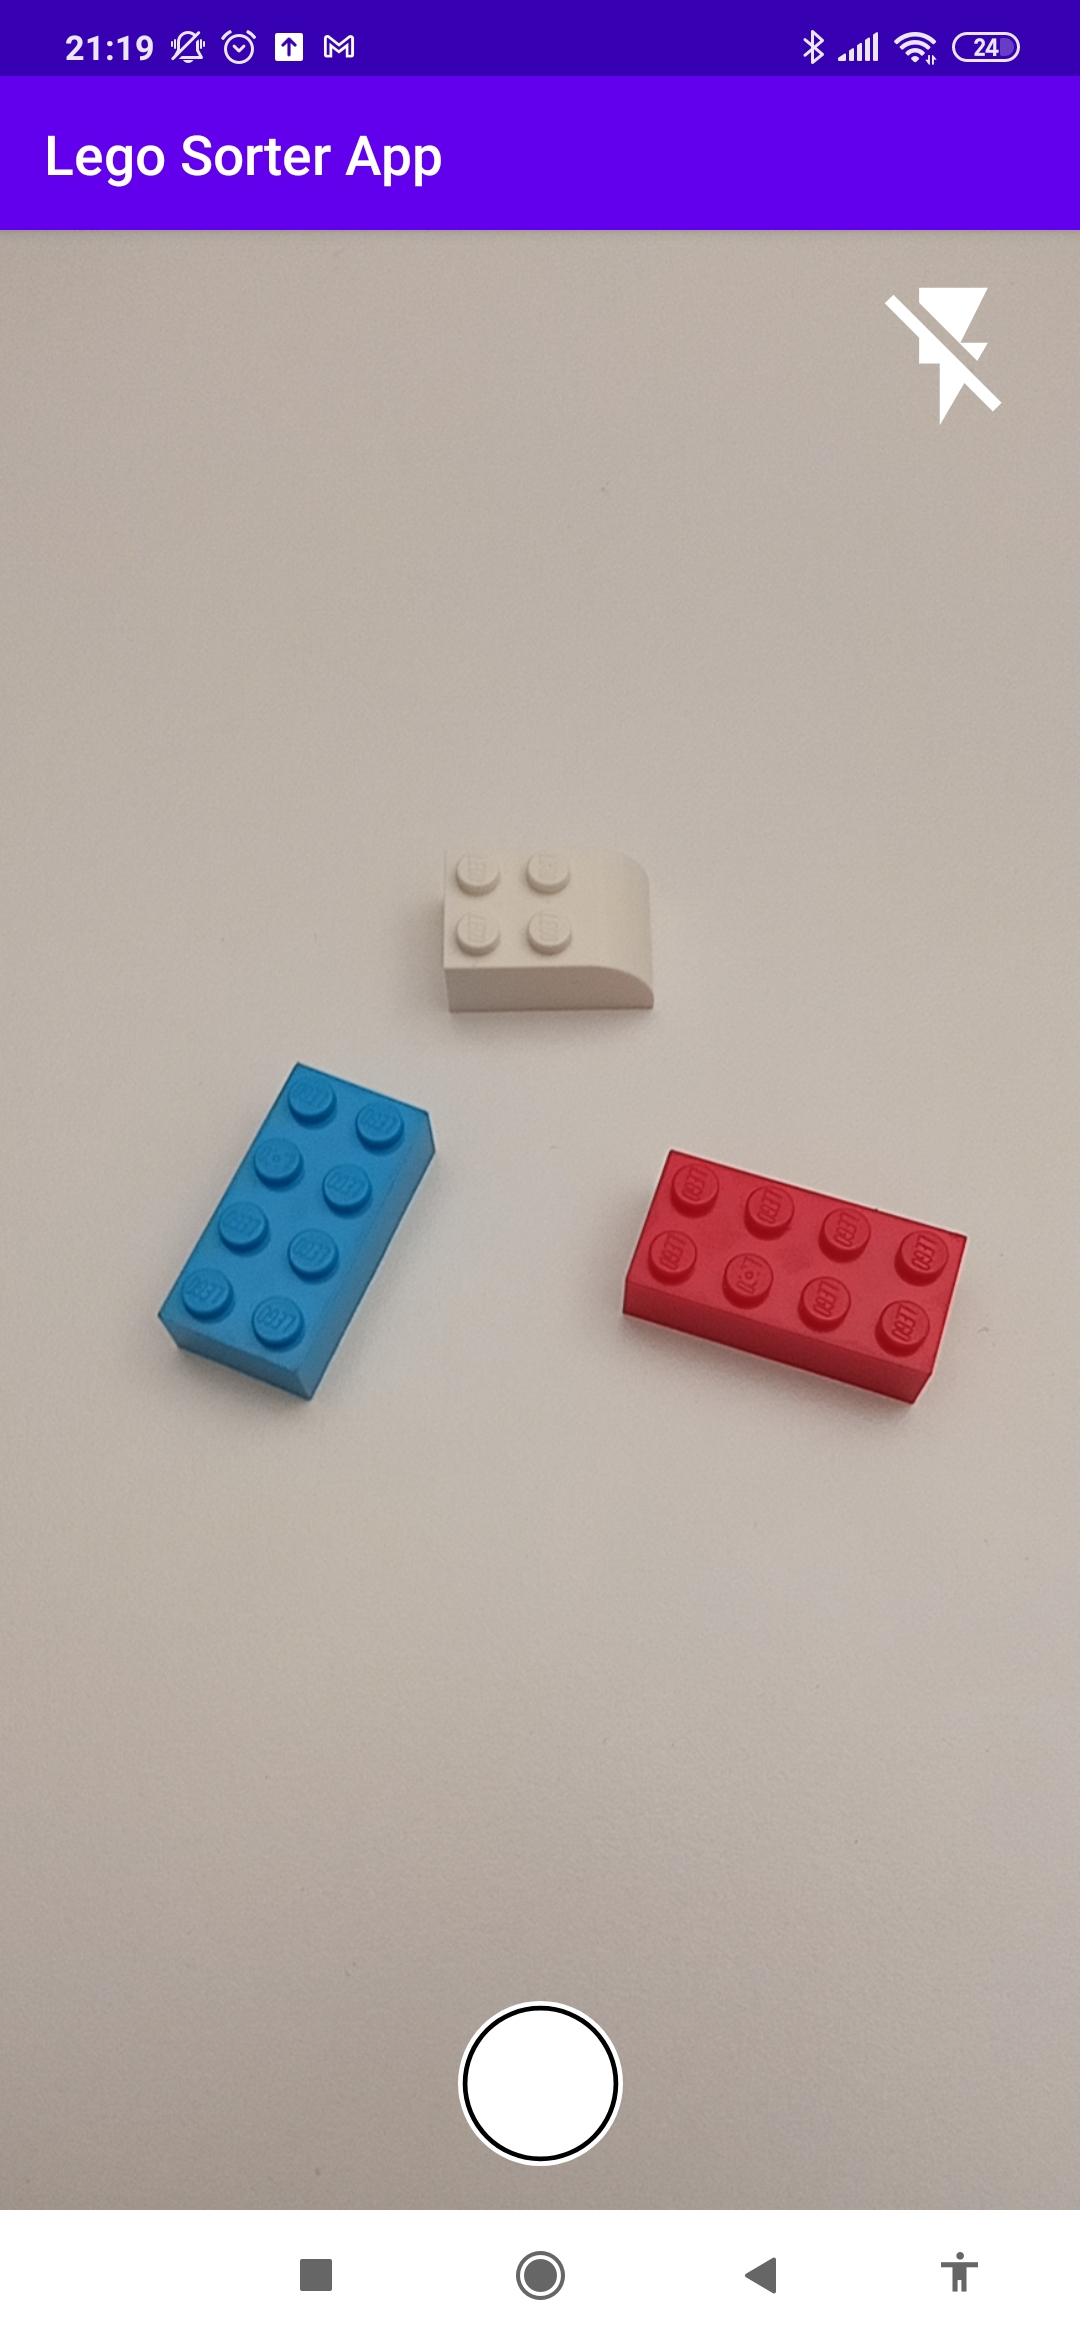
\includegraphics[width=0.3\linewidth]{capture_view}
		\centering
		\caption{Dodatkowo, tryb capture pozwala na włączenie opcji flasha i wykonywanie zdjęć ręcznie}
	\end{figure}
	
	
	\clearpage 
	\section{Serwer}
	Serwer jest odpowiedzialny za obsługę metod wywoływanch przez aplikację.
	\subsection{Przepływ sterowania}
	Tutaj opisać jak to jest wszystko wywoływane, napisać, że najpierw detekcja, potem klasyfikacja
	\subsection{gRPC}
	\subsection{Kolejkowanie zapytań}
	\subsection{Zapisywanie zdjęć}
	\newpage
	\section{Detekcja klocków}
	Kluczowym krokiem do rozpoznania klocków na zdjęciu jest ich zlokalizowanie. Możliwość detekcji klocków na zdjęciu rozszerza funkcjonalności, które jesteśmy w stanie dostarczyć realizując ten projekt. 
	Przede wszystkim, analizowane zdjęcie może zawierać więcej niż jeden klocek lego, ponadto, na zdjęciu mogą znajdować się inne przedmioty. 
	\par
	W idealnym przypadku, gdy klocek jest na równooświetlonej, białej powierzchni,
	możliwe jest wykrycie pozycji klocka z użyciem openCV, poprzez analizę kolorów
	na zdjęciu, jednak to rozwiązanie zawodzi w środowisku bez równego oświetlenia i ze zmiennym tłem, co nie pozwala na rozwiązanie tego problemu w prosty sposób.
	Przy użyciu sieci neuronowej możliwe jest wyeliminowanie powyższych problemów i wytrenowanie sieci w taki sposób, by znajdowała klocek na dowolnej powierzchni z ignorowaniem innych obiektów. Dzięki temu rozwiązaniu będzie możliwe szybkie generowanie datasetu z klockami Lego oraz skuteczniejszą naukę klasyfikacji klocków w oddzielnej sieci.
	
	\begin{figure}[h!]
		\centering
		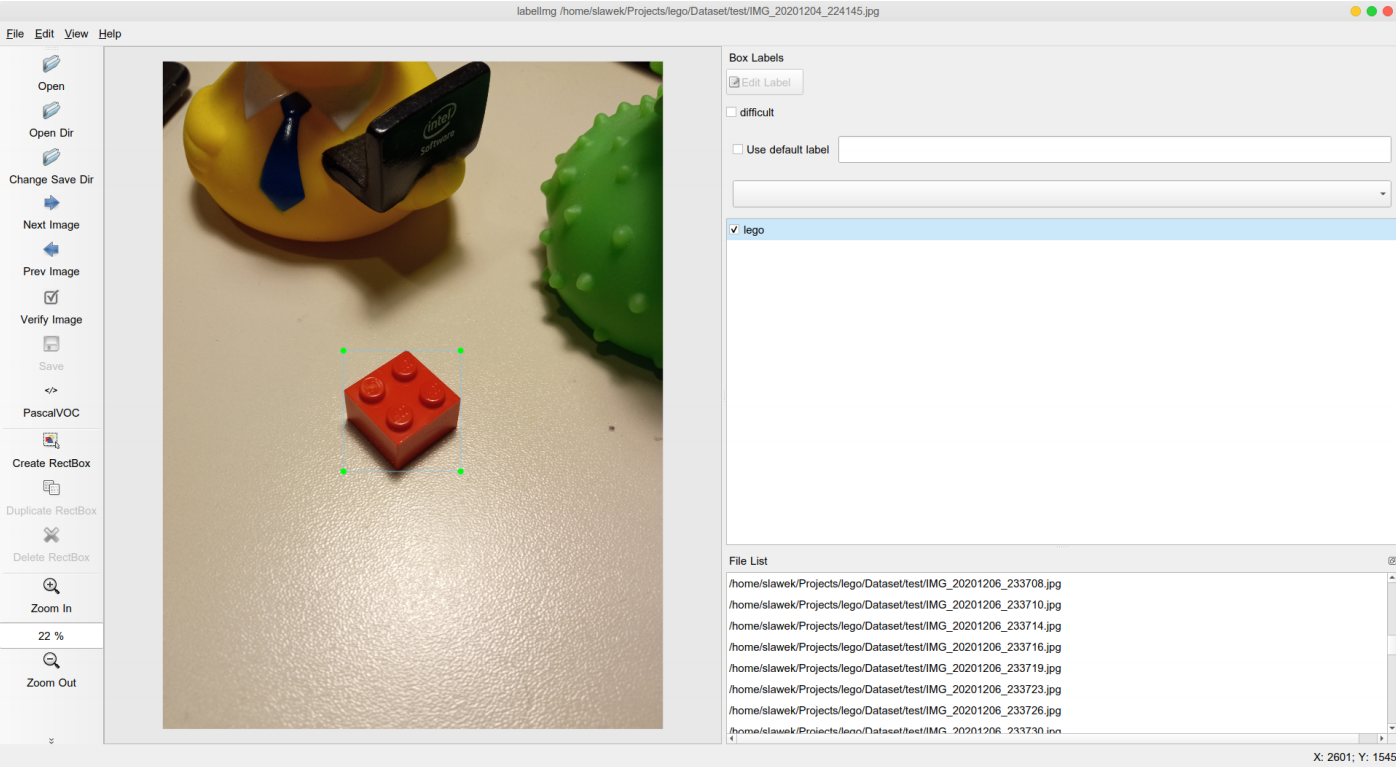
\includegraphics[width=0.7\linewidth]{images/detection_1}
		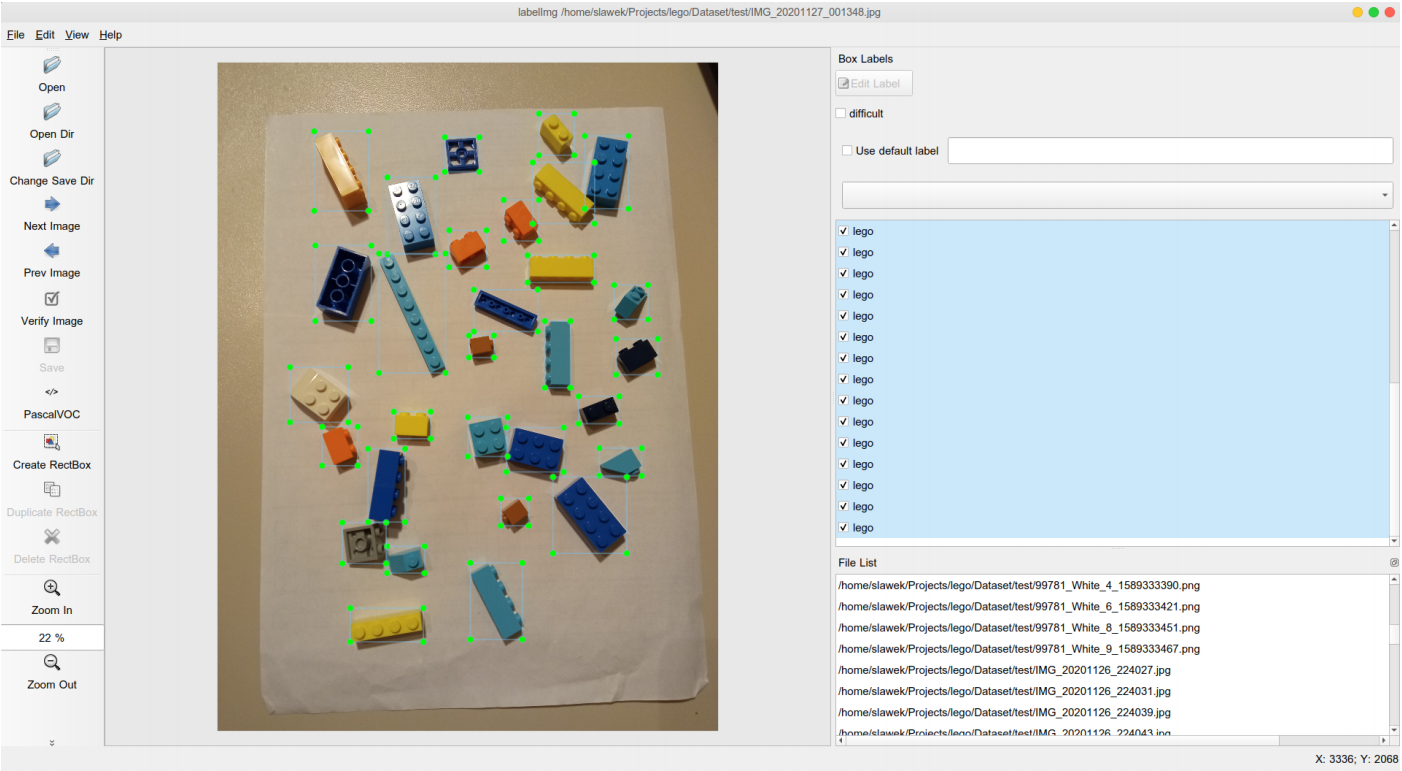
\includegraphics[width=0.7\linewidth]{images/detection_2}	
		\caption{Proces przygotowywania datasetu dla detekcji klocków}
	\end{figure}
	
	\par
	Warto zaznaczyć, że sieć będzie wykrywała tylko jedną klasę “Lego“ bez rozróżnienia jakiego typu jest znaleziony klocek.
	Głównymi powodami tej decyzji jest względnie duża liczba klas klocków Lego,
	przekraczająca 20 tysięcy oraz artykuł opisujący podobne rozwiązanie - detekcję
	ogólnej klasy i klasyfikacja dokładnej klasy - https://arxiv.org/abs/2001.09203
	
	
	\par W chwili pisania tego raportu, zbiór zdjęć do nauki detekcji liczy około 4300 ręcznie opisanych zdjęć, przy czym ponad połowa zdjęć to zdjęcia rzeczywistych klocków, natomiast resztę stanowią opisane rendery. 
	
	\section{Rozpoznawanie klocków}
	
\end{document}
